\documentclass{article}

\usepackage{amsmath, amssymb}
\usepackage[utf8]{inputenc}
\usepackage{geometry}
\usepackage{tikz}
\usetikzlibrary{arrows.meta}
\usetikzlibrary{fit}
\usetikzlibrary{positioning}
\usepackage{xr}
\externaldocument[proof:]{proofs}

\begin{document}
\section{List Of Models}
\subsection{Infinite Words}
\begin{itemize}
	\item DBA
	\item NBA
	\item GBA
	\item Rabin automaton
	\item Muller automaton
	\item Parity automaton
	\item det. E automaton
	\item det. A automaton
	\item det. coBA
	\item weak BA
	\item Staiger-Wagner automaton
	\item ABA
	\item LTL
	\item S1S
	\item $\exists$S1S
	\item S1S\textsubscript{0}
\end{itemize}

\subsection{Finite Trees}
\begin{itemize}
	\item DTA
	\item NTA
	\item $\downarrow$DTA
	\item $\downarrow$NTA
	\item DUTA
	\item NUTA
	\item deterministic DTD
	\item DTD
	\item deterministic EDTD
	\item single-type EDTD
	\item EDTD
	\item Relax NG
	\item FO
	\item MSO
	\item Regular expressions
	\item DTWA
	\item TWA
\end{itemize}

\subsection{Infinite Trees}
\begin{itemize}
	\item BTA
	\item Muller TA
	\item Parity TA
	\item DMTA
	\item S2S (MSO / WMSO)
	\item S2S\textsubscript{0} (MSO / WMSO)
\end{itemize}

\section{List Of Games}
\begin{itemize}
	\item Büchi
	\item Staiger-Wagner
	\item weak Parity
	\item Reachability
	\item Safety
	\item Muller
	\item Parity
	\item Rabin
	\item Streett
	\item Gale-Stewart
	\item Wadge
\end{itemize}

\newpage

\section{Infinite Word Models}
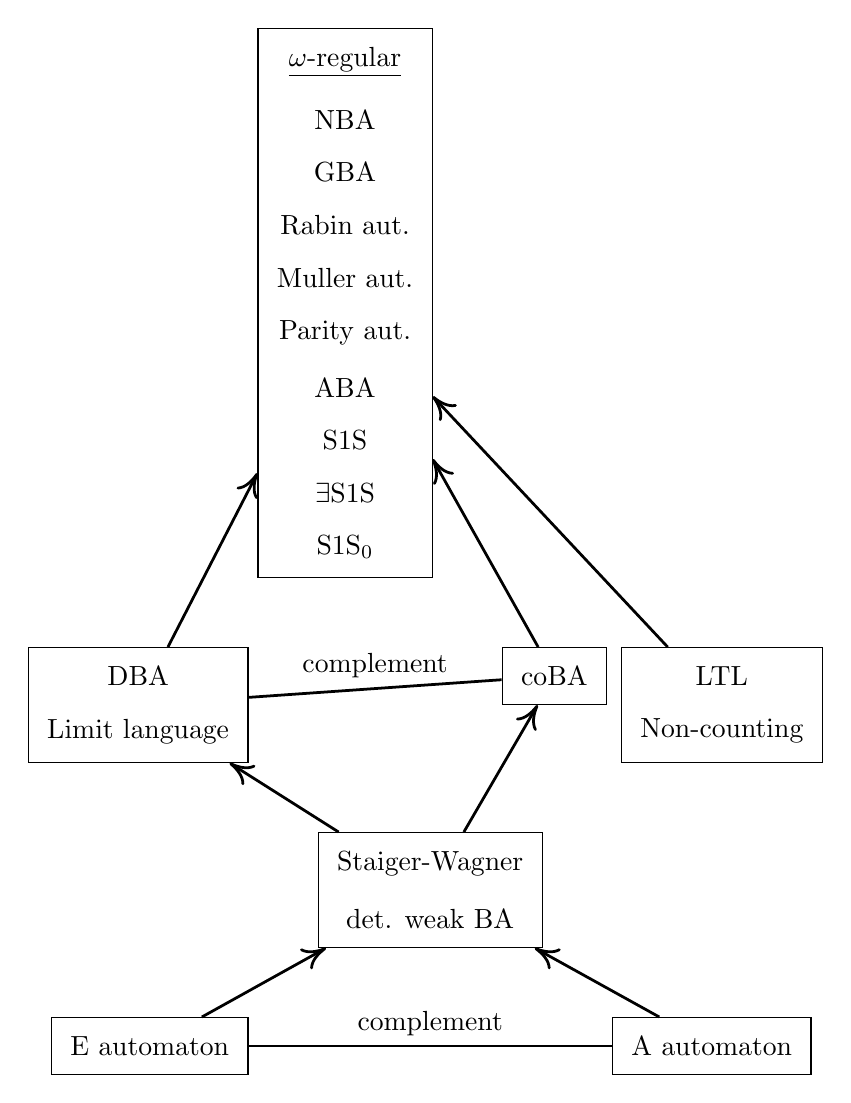
\begin{tikzpicture}
  \node (ireg) {\underline{$\omega$-regular}};
  \node (iNBA) [below=5pt of ireg] {NBA};
  \node (iGBA) [below=5pt of iNBA] {GBA};
  \node (iRabin) [below=5pt of iGBA] {Rabin aut.};
  \node (iMuller) [below=5pt of iRabin] {Muller aut.};
  \node (iParity) [below=5pt of iMuller] {Parity aut.};
  \node (iABA) [below=5pt of iParity] {ABA};
  \node (iS1S) [below=5pt of iABA] {S1S};
  \node (iES1S) [below=5pt of iS1S] {$\exists$S1S};
  \node (iS1S0) [below=5pt of iES1S] {S1S\textsubscript{0}};
  \node [draw, fit={(ireg) (iNBA) (iGBA) (iRabin) (iMuller) (iParity) (iABA) (iS1S) (iES1S) (iS1S0)}] (c1) {};
  
  \node (iDBA) [below left=of c1] {DBA};
  \node (ilimit) [below=5pt of iDBA] {Limit language};
  \node [draw, fit={(iDBA) (ilimit)}] (c2) {};
  
  \node (icoBA) [below right=of c1] {coBA};
  \node [draw, fit={(icoBA)}] (c3) {};
  
  \node (iSW) [below right=of c2] {Staiger-Wagner};
  \node (iweakBA) [below=5pt of iSW] {det. weak BA};
  \node [draw, fit={(iSW) (iweakBA)}] (c4) {};
  
  \node (iLTL) [right=of c3] {LTL};
  \node (inonc) [below=5pt of iLTL] {Non-counting};
  \node [draw, fit={(iLTL) (inonc)}] (c5) {};
  
  \node (iEA) [below left=of c4] {E automaton};
  \node [draw, fit={(iEA)}] (c6) {};
  
  \node (iAA) [below right=of c4] {A automaton};
  \node [draw, fit={(iAA)}] (c7) {};
  
   \draw [-{>[length=3mm,width=3mm]}, line width=1pt] (c2) -- (c1);
   \draw [-{>[length=3mm,width=3mm]}, line width=1pt] (c3) -- (c1);
   \draw [-{>[length=3mm,width=3mm]}, line width=1pt] (c5) -- (c1);
   \draw [-{>[length=3mm,width=3mm]}, line width=1pt] (c4) -- (c2);
   \draw [-{>[length=3mm,width=3mm]}, line width=1pt] (c4) -- (c3);
   \draw [-{>[length=3mm,width=3mm]}, line width=1pt] (c6) -- (c4);
   \draw [-{>[length=3mm,width=3mm]}, line width=1pt] (c7) -- (c4);
   \draw [-, line width=1pt] (c2) -- node [midway,above] {complement} (c3);
   \draw [-, line width=1pt] (c6) -- node [midway,above] {complement} (c7);
\end{tikzpicture}

\subsection{Class Inclusions}
\begin{itemize}
	\item E aut. $\subseteq$ Staiger-Wagner \\
		\textbf{Proof}: SWA with $\mathcal{F} = \{ Q' \subseteq Q \mid F \cap Q' \neq \emptyset \}$.
    \item A. aut. $\subseteq$ Staiger-Wagner \\
    	\textbf{Proof}: SW closed under complement,
    \item Staiger-Wagner $\subseteq$ DBA / coBA \\
    	\textbf{Proof}: $\mathcal{A}$ SWA $\Rightarrow$ $\mathcal{A}' = (Q \times 2^Q, \Sigma, (q_0, \emptyset), \delta', F')$ \\
    	Collect all visited states and accept if that set stays in $\mathcal{F}$.
    \item DBA $\subseteq$ NBA \\
    	trivial
    \item coBA $\subseteq$ NBA \\
    	\textbf{Proof}: NBA closed under complement.
    \item LTL $\subseteq$ NBA \\
    	\textbf{Proof}: \ref{} %TODO 6
    \item LTL $\subseteq$ ABA \\
    	\textbf{Proof}: \ref{} %TODO 21-22
\end{itemize}

\subsection{Class Exclusions}
\begin{itemize}
	\item E aut. $\not\subseteq$ A aut. \\
		\textbf{Example}: $b^* a (a+b)^\omega$ \\
    	\textbf{Proof}: Assume the A automaton $\mathcal{A} = (Q, \Sigma, q_0, \delta, F)$ recognizes $L$, so for every $b^n a b^\omega$, the run $\rho_n$ is accepting. Let $\rho^*(n) = \rho_{n+1}(n)$. This is an accepting run on $b^\omega$, which is a contradiction.
	\item A aut. $\not\subseteq$ E aut. \\
		\textbf{Example}: $\{a^\omega\}$ \\
    	\textbf{Proof}: Assume the E automaton $\mathcal{A} = (Q, \Sigma, q_0, \delta, F)$ recognizes $L$, so the run $\rho$ of $\mathcal{A}$ on $a^\omega$ is accepting. That means there is an $n$ s.t. $\rho(n) \in F$. Therefore, $\mathcal{A}$ accepts the word $a^n b^\omega$, which is a contradiction.
	\item DBA $\not\subseteq$ coBA \\
		\textbf{Example}: $(a^*b)^\omega$ \\
    	\textbf{Proof}: Assume $\mathcal{A} = (Q, \Sigma, q_0, \delta, F)$ is a coBA recognizing $L$. Let $n = |Q|$, $w = (a^n b)^\omega$, and $\rho$ the run of $\mathcal{A}$ on $w$. From some $m$ on, $\rho$ only visits states in $F$. Consider $(a^n b)^m a^n$. By choice of $n$, there must be $i < j$ such that after $(a^n b)^m a^i$ and $(a^n b)^m a^j$, the automaton is in the same state $q \in F$. Therefore, the run on $(a^n b)^m a^\omega$ is accepting, which is a contradiction.
	\item coBA $\not\subseteq$ DBA \\
		\textbf{Example}: $(a+b)^* a^\omega$ \\
    	\textbf{Proof}: Assume $\mathcal{A} = (Q, \Sigma, q_0, \delta, F)$ is a DBA recognizing $L$. We inductively define words $w_n$ with runs $\rho_n$ s.t. $w_n \sqsubseteq w_{n+1}$ and $\rho_n$ visits $F$ at least $n$ times and $|w_n|_b = n$. Then the ``limit'' of those words contains infinitely many $b$ but is accepted by $\mathcal{A}$, which is a contradiction. \\
    	Let $w_0 = \varepsilon$ and $\rho_0 = q_0$. For $n+1$, consider $w_n a^\omega$ with the run $\rho_n \pi$. Since $w_n a^\omega \in L$, there is a $k$ s.t. $\pi(k) \in F$. Let $w_{n+1} = w_n a^k b$ and $\rho_{n+1}$ accordingly.
	\item LTL $\not\subseteq$ NBA \\
		\textbf{Example}: $((a+b) a)^\omega$ \\
    	\textbf{Proof}: Show that $L$ is counting. Then it follows that it is not LTL-definable. Assume that $L$ is non-counting, so there is an $n_0$ according to the definition. Let $n = n_0 + 1$, $u = \varepsilon$, $v = a$, and $\beta = b a^\omega$. Due to symmetry, we can assume that $n_0$ is even, so $u v^n \beta \notin L$ but $u v^{n+1} \beta \in L$.
\end{itemize}

\subsection{Class Equalities}
\subsubsection{NBA}
\begin{itemize}
	\item NBA $\Leftrightarrow$ $\omega$-regular \\
    	\textbf{Proof}: \ref{} %TODO F3
	\item GBA $\Rightarrow$ NBA \\
    	\textbf{Proof}: \ref{} %TODO F3
    \item NBA $\Rightarrow$ $\exists$S1S \\
    	\textbf{Proof}: \ref{} %TODO F9
    \item S1S $\Rightarrow$ S1S\textsubscript{0} \\
    	\textbf{Proof}: \ref{} %TODO F9
    \item S1S\textsubscript{0} $\Rightarrow$ NBA \\
    	\textbf{Proof}: \ref{} %TODO F10
    \item Det. Muller $\Rightarrow$ NBA \\
    	\textbf{Proof}: NBA with $L(\mathcal{A}) = \bigcup\limits_{F \in \mathcal{F}} \left( \bigcap\limits_{q \in F} L(\mathcal{A}_q) \cap \bigcap\limits_{q \notin F} \overline{L(\mathcal{A}_q)} \right)$ where $\mathcal{A}_q$ is $\mathcal{A}$ starting in $q$.
    \item NBA $\Rightarrow$ det. Muller \\
    	\textbf{Proof}: \ref{} %TODO F12
   	\item (det.) Muller $\Rightarrow$ (det.) Parity \\
   		\textbf{Proof}: \ref{} %TODO F14
   	\item ABA $\Rightarrow$ NBA \\
   		\textbf{Proof}: \ref{} %TODO F23
\end{itemize}

\subsubsection{LTL}
LTL $\Leftrightarrow$ Non-counting \\
No proof. Remarks in F8.

A language $L$ is called \textbf{non-counting} if there is an $n_0$ such that for all $n > n_0$, all $u, v \in \Sigma^*$, and all $\beta \in \Sigma^\omega$: $uv^n\beta \in L \leftrightarrow uv^{n+1}\beta \in L$.

\subsubsection{SW}
Staiger-Wagner $\Leftrightarrow$ det. weak BA \\
\textbf{Proof}: \ref{} %TODO F18

\subsection{Closures}
\subsubsection{NBA}
\begin{itemize}
	\item Closed under union \\
    	\textbf{Proof}: Product automaton with $F = (F_1 \times Q_2) \cup (Q_1 \times F_2)$.
    \item Closed under intersection \\
    	\textbf{Proof}: GBA $\mathcal{A} = (Q_1 \times Q_2, \Sigma, (q_0^1, q_0^2), \Delta, (F_1 \times Q_2, Q_1 \times F_2))$ where \\
    	$\Delta = \{ ((p_1, p_2), a, (q_1, q_2)) \mid (p_1, a, q_1) \in \Delta_1, (p_2, a, q_2) \in \Delta_2 \}$.
    \item Closed under complement \\
    	\textbf{Proof}: \ref{} %TODO F4
\end{itemize}

\subsubsection{DBA}
\begin{itemize}
	\item Not closed under complement (inf. many $a$ $\leftrightarrow$ fin. many $a$)
\end{itemize}

\subsubsection{SW}
\begin{itemize}
	\item Closed under union and intersection \\
    	\textbf{Proof}: Product automaton with $\mathcal{F}_\cap = \{ F \subseteq Q_1 \times Q_2 \mid \pi_1(F) \in \mathcal{F}_1, \pi_2(F) \in \mathcal{F}_2 \}$ where $\pi_i((x_1, x_2)) = x_1$. 
    \item Closed under complement \\
    	\textbf{Proof}: $\overline{\mathcal{F}} = 2^Q \setminus \mathcal{F}$.
\end{itemize}

\subsection{Characterizations}
\begin{itemize}
	\item Parity conditions are directly convertible to Rabin chain conditions and vice-versa. \\
		\textbf{Proof}: Assign priorities in ascending order; $E_k \rightarrow 0$, $F_k \setminus E_k \rightarrow 1$, $E_{k-1} \setminus F_k \rightarrow 2$ \dots
	\item $U$ is $\omega$-regular iff $U$ is a Boolean combination of DBA-languages \\
		\textbf{Proof}: NBAs are closed under Boolean operations. %TODO other direction
	\item $U$ is DBA-recog. iff $U = \text{lim}(L)$ for some regular $L \subseteq \Sigma^*$. \\
		\textbf{Proof}: \ref{} %TODO F2
	\item $U$ is E-recog. iff $U = L \cdot \Sigma^*$ for some regular $L \subseteq \Sigma^*$. \\
		\textbf{Proof}: \ref{} %TODO F16
	\item Landweber's theorem \\
		\textbf{Proof}: \ref{} %TODO F16-F18
	\item DBA $\cap$ coBA $\Rightarrow$ SW \\
		\textbf{Proof}: \ref{} %TODO F18
\end{itemize}

\subsection{Duality}
\begin{itemize}
	\item $U$ is A-recog. iff $\Sigma^\omega \setminus U$ is E-recog. \\
		\textbf{Proof}: \ref{} %TODO F16
	\item $U$ is coBA-recog. iff $\Sigma^\omega \setminus U$ is DBA-recog. \\
		\textbf{Proof}: \ref{} %TODO F16
\end{itemize}

\subsection{Problems / Complexity}
\begin{itemize}
	\item Emptiness problem for NBAs is decidable in poly. time. \\
    	\textbf{Proof}: \ref{} %TODO F4
    \item Emptiness problem for ABAs is PSPACE-complete. \\
    	No proof. Remarks in F23.
    \item Membership problem for ABAs is decidable in poly. time. \\
    	%TODO F23;  infinite games?
\end{itemize}


\newpage

\section{Finite Tree Models}
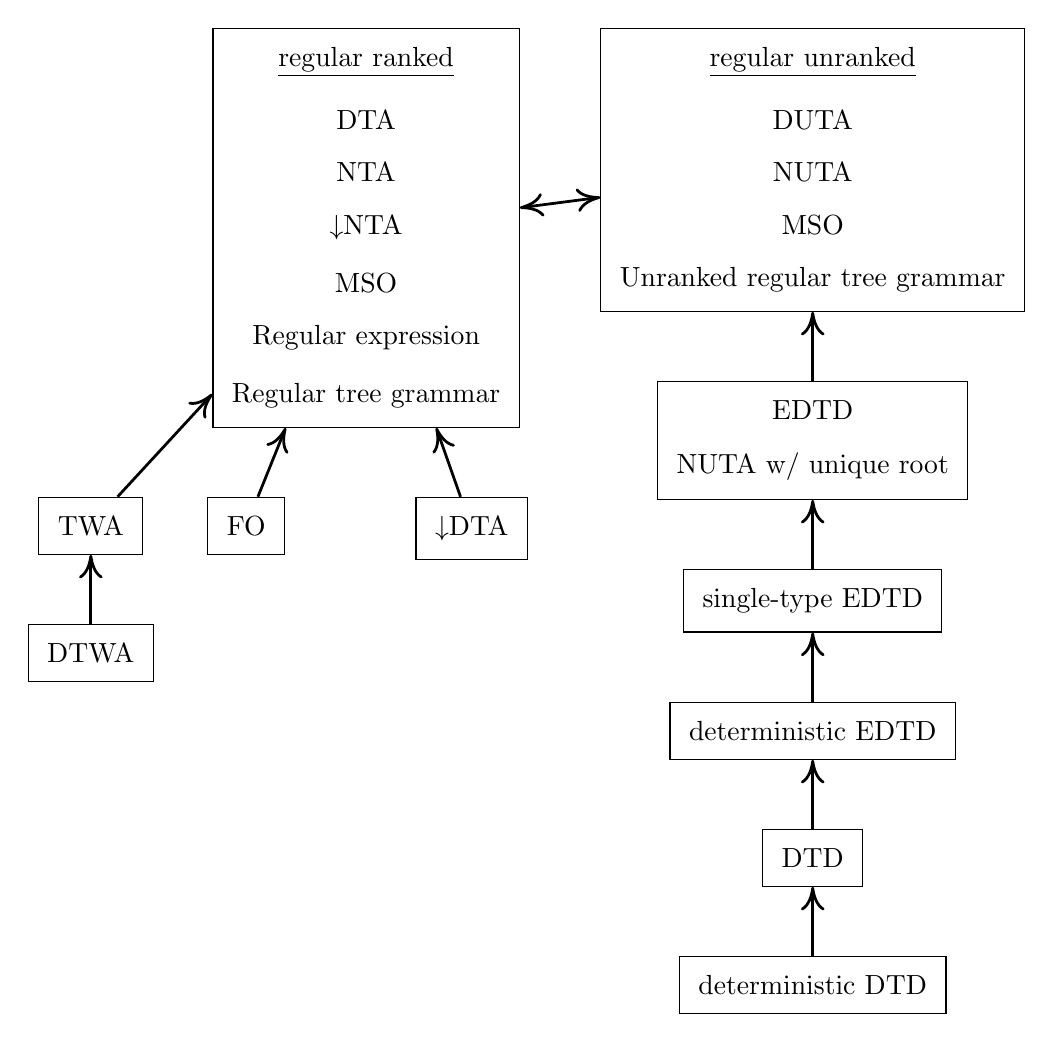
\begin{tikzpicture}
  \node (ireg) {\underline{regular ranked}};
  \node (iDTA) [below=5pt of ireg] {DTA};
  \node (iNTA) [below=5pt of iDTA] {NTA};
  \node (idNTA) [below=5pt of iNTA] {$\downarrow$NTA};
  \node (iMSO) [below=5pt of idNTA] {MSO};
  \node (iRegex) [below=5pt of iMSO] {Regular expression};
  \node (iRegGram) [below=5pt of iRegex] {Regular tree grammar};
  \node [draw, fit={(ireg) (iDTA) (iNTA) (idNTA) (iMSO) (iRegex) (iRegGram)}] (c1) {};
  
  \node (iregu) [right=3cm of ireg] {\underline{regular unranked}};
  \node (iDUTA) [below=5pt of iregu] {DUTA};
  \node (iNUTA) [below=5pt of iDUTA] {NUTA};
  \node (iMSOu) [below=5pt of iNUTA] {MSO};
  \node (iuRegGram) [below=5pt of iMSOu] {Unranked regular tree grammar};
  \node [draw, fit={(iregu) (iDUTA) (iNUTA) (iMSOu) (iuRegGram)}] (c2) {};
  
  \node (idDTA) [below right=1cm and -1.2cm of c1] {$\downarrow$DTA};
  \node [draw, fit={(idDTA)}] (c3) {};
  
  \node (iFO) [below left=1cm and -0.8cm of c1] {FO};
  \node [draw, fit={(iFO)}] (c8) {};
  
  \node (iEDTD) [below=of c2] {EDTD};
  \node (iNUTAsF) [below=5pt of iEDTD] {NUTA w/ unique root};
  \node [draw, fit={(iEDTD) (iNUTAsF)}] (c4) {};
  
  \node (istEDTD) [below=of c4] {single-type EDTD};
  \node [draw, fit={(istEDTD)}] (c5) {};
  
  \node (idEDTD) [below=of c5] {deterministic EDTD};
  \node [draw, fit={(idEDTD)}] (c6) {};
  
  \node (iDTD) [below=of c6] {DTD};
  \node [draw, fit={(iDTD)}] (c7) {};
  
  \node (idDTD) [below=of c7] {deterministic DTD};
  \node [draw, fit={(idDTD)}] (c11) {};
  
  \node (iTWA) [below left= of c1] {TWA};
  \node [draw, fit={(iTWA)}] (c9) {};
  
  \node (iDTWA) [below=of c9] {DTWA};
  \node [draw, fit={(iDTWA)}] (c10) {};
  
  \draw [{<[length=3mm,width=3mm]}-{>[length=3mm,width=3mm]}, line width=1pt] (c1) -- (c2);
  \draw [-{>[length=3mm,width=3mm]}, line width=1pt] (c3) -- (c1);
  \draw [-{>[length=3mm,width=3mm]}, line width=1pt] (c8) -- (c1);
  \draw [-{>[length=3mm,width=3mm]}, line width=1pt] (c4) -- (c2);
  \draw [-{>[length=3mm,width=3mm]}, line width=1pt] (c5) -- (c4);
  \draw [-{>[length=3mm,width=3mm]}, line width=1pt] (c6) -- (c5);
  \draw [-{>[length=3mm,width=3mm]}, line width=1pt] (c7) -- (c6);
  \draw [-{>[length=3mm,width=3mm]}, line width=1pt] (c11) -- (c7);
  \draw [-{>[length=3mm,width=3mm]}, line width=1pt] (c9) -- (c1);
  \draw [-{>[length=3mm,width=3mm]}, line width=1pt] (c10) -- (c9);
\end{tikzpicture}

\subsection{Class Inclusions}
\begin{itemize}
	\item Regular Ranked $\subseteq$ Regular Unranked \\
		\textbf{FCNS}: Let $\Sigma$ be an unranked alphabet. We define $\Gamma_0 = \{\#\}$ and $\Gamma_2 = \Sigma$. Let\linebreak $\overline{t} = t_1 \dots t_n \in T_\Sigma^*$ with $t_1 = a(t'_1 \dots t'_m)$. We define 
		$$\text{fcns}(\overline{t}) = \begin{cases}
			\# & \text{if } n = 0 \\
			a(\text{fcns}(t'_1, \dots, t'_m), \text{fcns}(t_2 \dots t_n)) & \text{else}
		\end{cases}$$
		
		See Theorem \ref{proof:fcns_correct}.
	\item det. DTD $\subseteq$ DTD $\subseteq$ det. EDTD $\subseteq$ single-type EDTD $\subseteq$ EDTD \\
		trivial
	\item EDTD $\subseteq$ Regular tree grammar \\
		\textbf{Proof}: $N = \Sigma'$, $P_\text{gram} = P \cup \{ a^{(n)} \rightarrow a \mid a, n\}$
	\item TWA $\subseteq$ NTA \\
		\textbf{Proof}: Theorem \ref{proof:twa_to_nta}
\end{itemize}

\subsection{Class Exclusions}
\begin{itemize}
	\item $\downarrow$DTA $\not\subseteq$ NTA \\
		\textbf{Example}: $T = \{ f(a, b), f(b, a) \}$ \\
		\textbf{Proof}: Assume the $\downarrow$DTA $\mathcal{A} = (Q, \Sigma, q_0, \Delta)$ accepts $T$. Let $(q_0, f, (q_1, q_2)) \in \Delta$, so also $(q_1, a), (q_1, b), (q_2, a), (q_2, b) \in \Delta$. However, that means the tree $f(a, a)$ is accepted by the run $q_0(q_1, q_2)$ which is a contradiction. On the other hand, NTAs can clearly recognize this property.
	\item DTD $\not\subseteq$ single-type EDTD \\
		\textbf{Example}: $T = \{ t \in T_{\{a,b\}} \mid \text{there is a path in } t \text{ on which } a \text{ occurs exactly twice}$
	\item NUTA w/ unique root $\not\subseteq$ NUTA \\
		\textbf{Example}: $T = \{a, b\}$
	\item FO $\not\subseteq$ MSO \\
		\textbf{Example}: $T = $ positive boolean terms that evaluate to true %F9
	\item DTWA $\not\subseteq$ TWA \\
		\textbf{Example}: $T_{N \backslash D}$ \\
			$\Sigma_0 = \{a, b\}$, $\Sigma_2 = \{f\}$ \\
			$t \in T_{N \backslash D}$ iff $|t|_a = 3 \land \text{lca}(u, v) \sqsubseteq \text{lca}(v, w)$
		\textbf{Proof}: DTWAs cannot recognize this tree language (no proof). TWAs can:
			\begin{itemize}
				\item Check whether there are exactly three $a$ and move to the right-most one (DFS).
				\item While going up, guess a node and go the the left-most ancestor.
				\item The tree is in $T_{N \backslash D}$ iff there are exactly two leafs labeled $a$ right of that node. (DFS)
			\end{itemize}
	\item TWA $\not\subseteq$ NTA \\
		\textbf{Example}: all paths in the skeleton have even length \\
		\textbf{Proof}: $\Sigma_0 = \{a, c\}$, $\Sigma_2 = \{b\}$ \\
			Skeleton of a tree $t$: replace all subtrees that contain exactly one $a$. \\
			TWAs cannot recognize this tree language (no proof). NTAs can (find ''merge`` points and count the parity)
\end{itemize}

\subsection{Class Equalities}
\subsubsection{Regular Ranked}
\begin{itemize}
	\item NTA $\Rightarrow$ DTA \\
		\textbf{Proof}: Subset construction.
	\item NTA $\Leftrightarrow$ $\downarrow$NTA \\
		\textbf{Proof}: Reverse the transitions and initial states $\leftrightarrow$ final states.
	\item $\downarrow$NTA $\Leftrightarrow$ Regular Tree Grammar \\
		\textbf{Proof}: Non-terminals correspond to states and transitions $(q, a, q_1, \dots, q_n)$ correspond to rules $A_q \rightarrow a(A_{q_1}, \dots, A_{q_n})$
	\item MSO $\Leftrightarrow$ NTA \\
		\textbf{Proof}: same as S2S
	\item Reg. exp. $\Leftrightarrow$ NTA \\
		\textbf{Proof}: Theorem \ref{proof:tre_fromto_nta}
\end{itemize}

\subsubsection{Regular Unranked}
\begin{itemize}
	\item NUTA $\Rightarrow$ DUTA \\
		\textbf{Proof}: Specialized subset construction. \\
		$\mathcal{A} = (Q, \Sigma, \Delta, F) \Rightarrow \mathcal{A}' = (2^Q, \Sigma, \Delta', \{P \subseteq Q \mid P \cap F \neq \emptyset\})$ \\
		$\Delta' = \{(L_{a,P}, a, P) \mid a \in \Sigma, P \subseteq Q\}$ with $L_{a,P} = \bigcap\limits_{p \in P} K_{a,p} \cap \bigcap\limits_{p \notin P} K_{a,p}^\complement$ \\
		$K_{a,p} = \{ P_1 \dots P_n \in (2^Q)^* \mid \exists p_1 \in P_1, \dots, p_n \in P_n: p_1 \dots p_n \in L_{a,p} \}$.
	\item MSO $\Leftrightarrow$ NUTA %no proof
\end{itemize}

\subsubsection{EDTD}
\begin{itemize}
	\item NUTA with unique root $\Leftrightarrow$ EDTD (in poly. time) \\
		\textbf{Proof}: $\boldsymbol{\Rightarrow}$ Let $q_0, \dots, q_n$ be an enumeration of $Q$. We then set $D = \{ \{ a^{(i)} \mid a \in \Sigma, 0 \leq i \leq n \}, P, a^{q_0})$ where $a$ is the unique root symbol of the automaton. Rules in $P$ guess arbitrary symbols for fitting states.
		
		$\boldsymbol{\Leftarrow}$ Analogously, we use $Q = \Sigma \times \{1, \dots, n\}$ where $n$ is the maximal type in $\Sigma'$ and rules mimic the transitions.
\end{itemize}

\subsection{Closures}
\subsubsection{Regular Ranked}
\begin{itemize}
	\item Regular (ranked) trees are closed under complement. \\
		\textbf{Proof}: Make $\Delta$ total (add sink state) and set $F' := Q \setminus F$.
	\item Regular (ranked) trees are closed under union and intersection. \\
		\textbf{Proof}: Product construction ($F_\cap = F_1 \times F_2$, $F_\cup = (Q_1 \times F_2) \cup (F_1 \times Q_2)$)
\end{itemize}

\subsubsection{Regular Unranked}
\begin{itemize}
	\item Regular unranked trees are closed under complement, union, and intersection. \\
		\textbf{Proof}: via FCNS, because ranked trees are closed under these operations
\end{itemize}

\subsubsection{TWA}
\begin{itemize}
	\item TWAs are closed under union. \\
		\textbf{Proof}: Non-deterministically choose at the start whether to execute $\mathcal{A}_1$ or $\mathcal{A}_2$.
	\item TWAs and DTWAs are closed under intersection. \\
		\textbf{Proof}: Execute $\mathcal{A}_1$. If it accepts, move to the root and execute $\mathcal{A}_2$.
	\item Open Problem: Are TWAs closed under complement?
	\item DTWAs are closed under complement. \\
		\textbf{Proof}: Theorem \ref{proof:dtwa_complement}
\end{itemize}


\subsection{Problems / Complexity}
\subsubsection{Regular Ranked}
\begin{itemize}
	\item Membership problem for NTAs is decidable.
	\item Reachable states of NTAs can be computed in linear time in $|\mathcal{A}|$.
		\textbf{Algorithm}: 
		\begin{enumerate}
			\item Initial reachable states $R = \{ q \in Q \mid \exists a \in \Sigma_0: (a, q) \in \Delta \}$
			\item For each transition $\tau = \{\overline{q}, a, p\} \in \Delta$, count $\text{in}(\tau) = |\overline{q}|$ and remember $\forall q \in \overline{q}: \tau \in \text{tr}(q)$.
			\item Grow $R$ by processing each reachable state once: Decrement $\text{in}(\tau)$ by 1; if that value reaches 0, every ingoing state of $\tau$ is reachable and therefore, the outgoing state is.
		\end{enumerate}
	\item Emptiness of an NTA can be decided in linear time in $|\mathcal{A}|$. \\
		\textbf{Algorithm}: $T(\mathcal{A}) = \emptyset$ iff $\text{Reachable}(\mathcal{A}) \cap F = \emptyset$
	\item Given a DTA $\mathcal{A}$, $\sim_{T(\mathcal{A})}$ can be computed in time $\text{poly}(|Q^m \times \Sigma \times Q|)$ where $m$ is the maximal arity in $\Sigma$. \\
		\textbf{Algorithm}: 
		\begin{enumerate}
			\item Mark all $(q, q')$ with $(q, q') \in (F \times Q \setminus F) \cup (Q \setminus F \times F)$.
			\item As long as there is still change in the marks, execute step 3:
			\item If $(p, p')$ is already marked and there are $q_1, \dots, q_{i-1}, q, q', q_{i+1}, \dots, q_n \in Q$ and $a \in \Sigma_n$ such that $p = \delta(q_1, \dots, q, \dots, q_n, a)$ and $p' = \delta(q_1, \dots, q', \dots, q_n, a)$, then mark the pair $(q, q')$. 
			\item $p \sim_{T(\mathcal{A})} q$ iff $(p, q)$ is not marked.
		\end{enumerate}
\end{itemize}

\subsubsection{Regular Unranked}
\begin{itemize}
	\item Emptiness / membership / inclusion for NUTAs is decidable in polynomial / polynomial / exponential time. \\
		\textbf{Algorithm} (Emptiness): Use FCNS transformation. \\
		\textbf{Algorithm} (Membership): Construct $\mathcal{A}_t$ with $T(\mathcal{A}_t) = \{t\}$ and check $\mathcal{A} \cap \mathcal{A}_t \overset{?}{=} \emptyset$. \\
		\textbf{Algorithm} (Inclusion): Check $T(\mathcal{A}_1) \cap T(\mathcal{A}_2)^\complement \overset{?}{=} \emptyset$. Complementation is exponential.
	\item Inclusion for complete DUTAs is decidable in polynomial time. \\
		\textbf{Algorithm}: Same algorithm as for general NUTAs but complementation can be done in polynomial time.
\end{itemize}

\subsubsection{Grammars}
\begin{itemize}
	\item Emptiness / membership for EDTDs is decidable in polynomial time. \\
		\textbf{Proof}: EDTD can be converted to NUTA in polynomial time.
	\item Inclusion for deterministic EDTDs is decidable in polynomial time. \\
		\textbf{Proof}: Let $D_1, D_2$ be deterministic EDTDs. Using the previous results and theorem \ref{proof:edtd_complto_nuta}, we can construct NUTAs $\mathcal{A}, \mathcal{B}$ with $T(\mathcal{A}) = T(D_1)$ and $T(\mathcal{B}) = T(D_2)^\complement$ in polynomial time. Then $T(D_1) \subseteq T(D_2)$ iff $T(\mathcal{A}) \cap T(\mathcal{B}) = \emptyset$.
\end{itemize}

\newpage

\section{Infinite Tree Models}
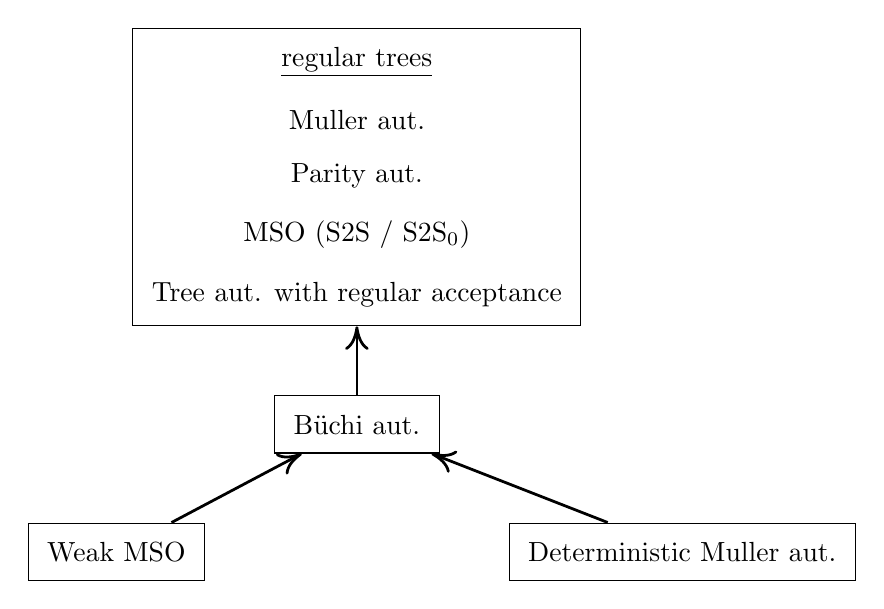
\begin{tikzpicture}
  \node (ireg) {\underline{regular trees}};
  \node (iMTA) [below=5pt of ireg] {Muller aut.};
  \node (iPTA) [below=5pt of iMTA] {Parity aut.};
  \node (iMSO) [below=5pt of iPTA] {MSO (S2S / S2S\textsubscript{0})};
  \node (iTAreg) [below=5pt of iMSO] {Tree aut. with regular acceptance};
  \node [draw, fit={(ireg) (iMTA) (iPTA) (iMSO) (iTAreg)}] (c1) {};
  
  \node (iBTA) [below=of c1] {Büchi aut.};
  \node [draw, fit={(iBTA)}] (c2) {};
  
  \node (iWMSO) [below left=of c2] {Weak MSO};
  \node [draw, fit={(iWMSO)}] (c3) {};
  
  \node (iDMTA) [below right=of c2] {Deterministic Muller aut.};
  \node [draw, fit={(iDMTA)}] (c4) {};
  
  \draw [-{>[length=3mm,width=3mm]}, line width=1pt] (c2) -- (c1);
  \draw [-{>[length=3mm,width=3mm]}, line width=1pt] (c3) -- (c2);
  \draw [-{>[length=3mm,width=3mm]}, line width=1pt] (c4) -- (c2);
\end{tikzpicture}

\subsection{Class Exclusions}
\begin{itemize}
	\item BTA $\not\subseteq$ Regular tree \\
		\textbf{Example}: $T_\text{fin} = \{ t \in T_{\{a,b\}} \mid \text{every infinite path has only fin. many } b \}$ \\
		\textbf{Proof}: %TODO F14
	\item DMTA $\not\subseteq$ BTA \\
		\textbf{Example}: $T_\text{fin}^\complement = \{ t \in T_{\{a,b\}} \mid \text{there is a path with inf. many } b \}$ \\
		\textbf{Proof}: BTA-recognizable (see below) but not a path tree language.
	\item WMSO $\not\subseteq BTA$ \\
		\textbf{Example}: $\{ t \in T_{\{a,b\}} \mid \text{every infinite path has infinitely many } b \}$ \\
		\textbf{Proof}: %TODO F19
\end{itemize}

\subsection{Class Equalities}
\subsubsection{Regular Trees}
\begin{itemize}
	\item PTA, MTA $\Rightarrow$ TA with regular acceptance \\
		\textbf{Proof}: By definition and PA/MA regularity.
	\item TA with reg. acc. $\Rightarrow$ PTA \\
		\textbf{Proof}: TA $\mathcal{A}$, DPA $\mathcal{A}'$ over alphabet $Q$ that defines Acc. Define PTA with state space $Q \times P$. \\
		$(q, a, q_1, q_2) \in \Delta \Rightarrow ((q,p), a, (q_1, \delta(p, q)), (q_2, \delta(p, q))) \in \Delta'$
	\item PTA $\Leftrightarrow$ MSO (S2S)
		\textbf{Proof}: \ref{} %TODO F18
\end{itemize}

\subsection{Closures}
\subsubsection{Regular Trees}
\begin{itemize}
	\item The class of regular tree languages is closed under union and intersection. \\
		\textbf{Proof}: \ref{} %TODO F15
	\item The class of regular tree languages is closed under projection. \\
		\textbf{Proof}: \ref{} %TODO F15
	\item PTAs are closed under complement ($2^{\mathcal{O}(kn \cdot \log(kn))}$ states for $|Q| = n$, $|\text{img}(c)| = k$)
		\textbf{Proof}: \ref{} %TODO F16-17
\end{itemize}

\subsubsection{BTA}
\begin{itemize}
	\item BTAs are not closed under complement. \\
		\textbf{Proof}: $T_\text{fin}^\complement = \{ t \in T_{\{a,b\}} \mid \text{there is a path with inf. many } b \}$ \\
		$T_\text{fin}^\complement$ is BTA-recognizable but its complement is not. %TODO F14
\end{itemize}

\subsubsection{DMTA}
\begin{itemize}
	\item DMTAs are not closed under union or complement. % no proof
	\item DMTAs are closed under intersection. \\
		\textbf{Proof}: product automaton
\end{itemize}

\subsection{Characterizations}
\begin{itemize}
	\item $T \subseteq T_\Sigma$ is DMTA-recognizable iff $T$ is a path tree language. \\
		$T : 2^{(\{0,1\} \times \Sigma)^\omega} \rightarrow 2^{T_\Sigma}, L \mapsto \{ t \in T_\Sigma \mid \forall \pi \in \{0,1\}^\omega: \pi^\smallfrown (t|_\pi) \in L \}$ \\
		\textbf{Proof}: %ex 9
	\item $T \subseteq T_\Sigma$ is WMSO-definable iff $T$ and $T^\complement$ are BTA-recognizable. % no proof
\end{itemize}

\subsection{Problems}
\subsubsection{Regular Trees}
\begin{itemize}
	\item The membership problem for regular tree languages is decidable. \\
		\textbf{Proof}: via membership game as in complementation
	\item The emptiness problem for regular tree languages is decidable. \\
		\textbf{Proof}: \ref{} %TODO F17
\end{itemize}


\end{document}
















